% Workstream xs results. Every number traces to data/research/flb_xs/ (summary.json, tables/*.json);
% tables are generated by `python -m albert.research.flb_xs run latex`.

This subsection measures the bias on Kalshi with the three measures of \cref{sec:method-xs}. The
benchmarks of \cref{sec:framework} guide the reading: a bias confined to the tick floor and the
no-arbitrage band points to mechanics, and a bias beyond them to preferences, information or beliefs.
Unless stated otherwise, statistics are market-weighted, pool the pre-event leads from 1 hour to
30 days, and use $t$-statistics clustered by event.

\subsubsection{Size of the bias}\label{sec:res-xs-size}

\paragraph{The bias is large per dollar and small per contract.}
\Cref{tab:xs-group} and \cref{fig:xs-calib,fig:xs-returns} give the headline.
\begin{itemize}
\item The calibration slope is $\hat\beta=\xsAllBeta$ ($t_{\beta=1}=\xsAllBetaT$): quoted odds are too
      moderate. This is the favourite--longshot bias familiar from racetracks
      \citep{griffith1949,thalerziemba1988,snowbergwolfers2010}.
\item Longshot sides return \xsAllLsMid\% per dollar at the mid ($t=\xsAllLsMidT$) and
      \xsAllLsNet\% net of spread and fees ($t=\xsAllLsNetT$).
\item Favourite sides return \xsAllFavMid\% per dollar at the mid ($t=\xsAllFavMidT$), but
      \xsAllFavNet\% at the ask after the fee ($t=\xsAllFavNetT$).
\item Volume weighting steepens the slope to $\hat\beta=\xsAllVolBeta$ ($t=\xsAllVolBetaT$) and
      deepens the longshot return to \xsAllVolLsMid\% at the mid ($t=\xsAllVolLsMidT$). In each of the
      six main groups the slope is steeper under volume weights (\xsGroupVolBetaMin{} to
      \xsGroupVolBetaMax, against \xsGroupBetaMin{} to \xsGroupBetaMax{} market-weighted).
\end{itemize}
The bias is concentrated in the tails (\cref{tab:xs-bucket}). In the 1--2\cents{} bucket, the mean
mid is \xsBOneQ\cents{} and the side wins \xsBOneWin\% of the time, a gross return of \xsBOneMid\% per
dollar ($t=\xsBOneMidT$). The 3--5\cents{} and 6--10\cents{} buckets return \xsBThreeMid\% and
\xsBSixMid\%. Between about 20\cents{} and 80\cents{} the realised frequency tracks the price, and no
bucket differs from zero by more than a few percent per dollar. At the top, the 99\cents{} bucket
earns \xsBNinetyNineMid\% at the mid ($t=\xsBNinetyNineMidT$) and \xsBNinetyNineNet\% net of the fee.
Per contract, these tails are small: the 1--2\cents{} bucket loses well under one cent. The large
per-dollar losses come from small prices, not from large errors in probability. \citet{burgi2025}
report a similar pattern in Kalshi trade prices.

\paragraph{YES bias.}
The intercept of the YES-side regression is $\hat\alpha=\xsAllAlpha$ ($t=\xsAllAlphaT$). A positive
$\hat\alpha$ means YES outcomes are slightly more frequent than YES prices imply, holding the slope fixed.
So within this sample, longshot losses are not driven by a preference for buying YES contracts.

\paragraph{Every category shows the bias.}
The longshot return at the mid is negative in every group, and the calibration slope is above one
in every group (\cref{tab:xs-group}). The differences between groups are modest.
\begin{itemize}
\item \emph{Entertainment} has the steepest slope ($\hat\beta=\xsEntBeta$, $t=\xsEntBetaT$),
      followed by \emph{Science \& Tech} ($\xsSciBeta$, $t=\xsSciBetaT$) and \emph{Weather}
      ($\xsWeatherBeta$, $t=\xsWeatherBetaT$).
\item \emph{Mentions} ($\xsMentionsBeta$, $t=\xsMentionsBetaT$), \emph{Sports} before the game
      ($\xsSportsBeta$, $t=\xsSportsBetaT$) and in play ($\xsInplayBeta$, $t=\xsInplayBetaT$), and
      \emph{Politics} ($\xsPoliticsBeta$, $t=\xsPoliticsBetaT$) are flatter.
\item The small \emph{Other} group (\xsOtherMkts{} markets: transport and similar) has
      $\hat\beta=\xsOtherBeta$.
\end{itemize}
Longshot returns rank the groups differently from the slope, because they also depend on how much
mass sits at the tick floor. Mentions longshots lose \xsMentionsLsMid\% per dollar
($t=\xsMentionsLsMidT$) and Weather longshots \xsWeatherLsMid\% ($t=\xsWeatherLsMidT$). Only
Entertainment stands out from the pooled slope by more than its sampling error. Sports and politics
are the groups with the most liquid external references, bookmaker lines and polls, and their
slopes are the lowest. That is consistent with an external anchor disciplining tail prices, but
the cross-group evidence is too weak to identify it. In baseball betting the bias is absent or
even reversed \citep{woodland1994}.

\begin{figure}[!htbp]
\centering
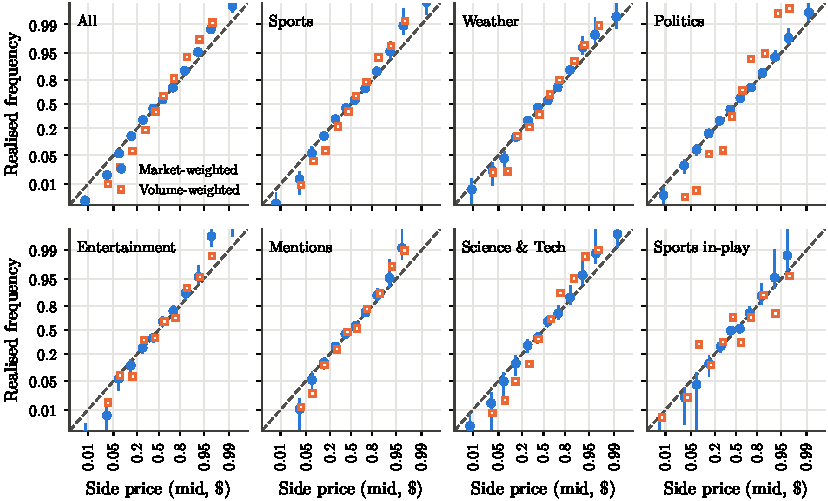
\includegraphics[width=\textwidth]{figures/fig_xs_calibration.pdf}
\caption{Calibration by group. Realised frequency of the side bought against its mid price, by
price bucket, on log-odds axes. Dots: market-weighted means with 95\% confidence intervals
clustered by event; open squares: volume-weighted (contracts traded in the 7 days to the quote).
Pre-event leads pooled; the last panel shows sports in-play quotes. The dashed line is perfect
calibration.}\label{fig:xs-calib}
\end{figure}

\begin{table}[!htbp]
\centering
\begin{threeparttable}
\caption{The favourite--longshot bias by group}\label{tab:xs-group}
\scriptsize
\setlength{\tabcolsep}{3pt}
\begin{tabular}{@{}lrrrrrrrrr@{}}
\toprule
% source: data/research/flb_xs/summary.json:measures_group
Group & Markets & Events & $\hat\beta$ & \LS & \FAV & \LS$-$\FAV & \LS & \FAV & \LS$-$\FAV \\
 & & & & \multicolumn{3}{c}{gross, at mid} & \multicolumn{3}{c}{net of taker fee, at ask} \\
\cmidrule(lr){5-7}\cmidrule(lr){8-10}
\midrule
\multicolumn{10}{@{}l}{\emph{A. Market-weighted}} \\
All groups & 19{,}007 & 4{,}770 & 1.129 & $-55.1$ & $+1.1$ & $-56.2$ & $-74.7$ & $-0.7$ & $-74.0$ \\
 &  &  & ($6.5$) & ($-10.0$) & ($9.8$) & ($-10.1$) & ($-25.3$) & ($-2.4$) & ($-24.1$) \\[2pt]
Sports & 6{,}284 & 1{,}521 & 1.099 & $-57.7$ & $+1.1$ & $-58.8$ & $-76.8$ & $-0.6$ & $-76.1$ \\
 &  &  & ($2.6$) & ($-4.3$) & ($4.8$) & ($-4.3$) & ($-11.0$) & ($-0.9$) & ($-10.6$) \\[2pt]
Weather & 2{,}901 & 1{,}065 & 1.152 & $-30.7$ & $+1.5$ & $-32.2$ & $-61.4$ & $-0.6$ & $-60.7$ \\
 &  &  & ($2.9$) & ($-1.4$) & ($4.0$) & ($-1.4$) & ($-5.2$) & ($-0.9$) & ($-5.0$) \\[2pt]
Politics & 3{,}906 & 968 & 1.075 & $-42.5$ & $+0.5$ & $-43.0$ & $-67.0$ & $-1.8$ & $-65.2$ \\
 &  &  & ($1.8$) & ($-4.5$) & ($2.2$) & ($-4.4$) & ($-12.2$) & ($-3.1$) & ($-11.3$) \\[2pt]
Entertainment & 2{,}665 & 530 & 1.254 & $-71.0$ & $+1.4$ & $-72.3$ & $-84.6$ & $-0.1$ & $-84.5$ \\
 &  &  & ($4.8$) & ($-8.2$) & ($6.9$) & ($-8.3$) & ($-18.7$) & ($-0.1$) & ($-17.6$) \\[2pt]
Mentions & 1{,}760 & 103 & 1.127 & $-75.8$ & $+1.6$ & $-77.4$ & $-85.0$ & $+0.5$ & $-85.5$ \\
 &  &  & ($2.0$) & ($-12.1$) & ($3.4$) & ($-11.6$) & ($-17.0$) & ($0.5$) & ($-15.3$) \\[2pt]
Science \& Tech & 1{,}375 & 510 & 1.175 & $-64.0$ & $+1.2$ & $-65.2$ & $-77.3$ & $-0.4$ & $-76.9$ \\
 &  &  & ($2.6$) & ($-6.0$) & ($3.7$) & ($-6.0$) & ($-11.0$) & ($-0.5$) & ($-10.1$) \\[2pt]
Other & 116 & 73 & 1.463 & $-95.2$ & $+2.9$ & $-98.1$ & $-95.7$ & $+3.2$ & $-98.9$ \\
 &  &  & ($2.4$) & ($-19.3$) & ($5.7$) & ($-18.2$) & ($-21.4$) & ($3.9$) & ($-19.0$) \\[2pt]
Sports in-play & 812 & 242 & 1.086 & $-74.1$ & $+1.4$ & $-75.5$ & $-82.3$ & $-0.1$ & $-82.2$ \\
 &  &  & ($1.1$) & ($-8.5$) & ($3.0$) & ($-8.3$) & ($-14.2$) & ($-0.1$) & ($-12.8$) \\[2pt]
\midrule
\multicolumn{10}{@{}l}{\emph{B. Volume-weighted (contracts traded in the 7 days to $t$)}} \\
All groups & 19{,}007 & 4{,}770 & 1.477 & $-85.6$ & $+1.6$ & $-87.3$ & $-90.5$ & $+1.8$ & $-92.3$ \\
 &  &  & ($3.6$) & ($-17.7$) & ($5.0$) & ($-17.6$) & ($-28.7$) & ($3.0$) & ($-25.8$) \\[2pt]
Sports & 6{,}284 & 1{,}521 & 1.373 & $-73.2$ & $+1.8$ & $-75.1$ & $-81.4$ & $+2.5$ & $-83.9$ \\
 &  &  & ($2.0$) & ($-5.6$) & ($3.2$) & ($-5.7$) & ($-9.7$) & ($1.9$) & ($-8.9$) \\[2pt]
Weather & 2{,}901 & 1{,}065 & 1.291 & $-81.0$ & $+1.3$ & $-82.3$ & $-87.2$ & $+2.1$ & $-89.3$ \\
 &  &  & ($2.0$) & ($-5.5$) & ($5.7$) & ($-5.5$) & ($-8.7$) & ($1.5$) & ($-7.9$) \\[2pt]
Politics & 3{,}906 & 968 & 1.795 & $-96.1$ & $+2.0$ & $-98.1$ & $-97.8$ & $+1.6$ & $-99.4$ \\
 &  &  & ($6.6$) & ($-67.0$) & ($2.6$) & ($-54.6$) & ($-120.7$) & ($6.0$) & ($-102.6$) \\[2pt]
Entertainment & 2{,}665 & 530 & 1.344 & $-85.3$ & $+0.9$ & $-86.2$ & $-90.7$ & $+0.3$ & $-91.0$ \\
 &  &  & ($3.0$) & ($-9.2$) & ($1.9$) & ($-8.9$) & ($-13.9$) & ($0.2$) & ($-11.7$) \\[2pt]
Mentions & 1{,}760 & 103 & 1.346 & $-92.0$ & $+1.4$ & $-93.4$ & $-93.6$ & $+2.1$ & $-95.7$ \\
 &  &  & ($4.6$) & ($-33.0$) & ($4.7$) & ($-31.6$) & ($-40.9$) & ($2.8$) & ($-33.3$) \\[2pt]
Science \& Tech & 1{,}375 & 510 & 1.564 & $-89.4$ & $+1.4$ & $-90.8$ & $-94.1$ & $+1.8$ & $-95.9$ \\
 &  &  & ($4.0$) & ($-22.4$) & ($6.8$) & ($-22.1$) & ($-39.5$) & ($3.4$) & ($-36.3$) \\[2pt]
Other & 116 & 73 & 1.431 & $-61.8$ & $+0.2$ & $-62.0$ & $-66.7$ & $+2.0$ & $-68.6$ \\
 &  &  & ($1.5$) & ($-1.5$) & ($0.1$) & ($-1.4$) & ($-1.9$) & ($0.5$) & ($-1.8$) \\[2pt]
Sports in-play & 812 & 242 & 0.810 & $+69.8$ & $-9.7$ & $+79.5$ & $+53.1$ & $-18.3$ & $+71.4$ \\
 &  &  & ($-0.6$) & ($0.5$) & ($-0.9$) & ($0.6$) & ($0.4$) & ($-1.2$) & ($0.5$) \\[2pt]
\bottomrule
\end{tabular}
\begin{tablenotes}\footnotesize
\item Pre-event quotes at leads of 1\,h to 30\,d before the scheduled time, pooled; sports in-play:
0.5--2\,h after the scheduled start. $\hat\beta$: slope of the logit regression~\eqref{eq:xs-logit},
with $t_{\beta=1}$ in parentheses. \LS, \FAV: mean return per dollar (\%) of sides priced at most
10\cents{} or at least 90\cents; \LS$-$\FAV: their difference. Gross: at the mid, no fee. Net: at the
ask, net of the exact taker fee, sides bucketed by the ask. Panel A gives each market weight one;
panel B weights quotes by contracts traded in the 7 days to the quote. $t$-statistics clustered
by event in parentheses.
\end{tablenotes}
\end{threeparttable}
\end{table}

\begin{figure}[!htbp]
\centering
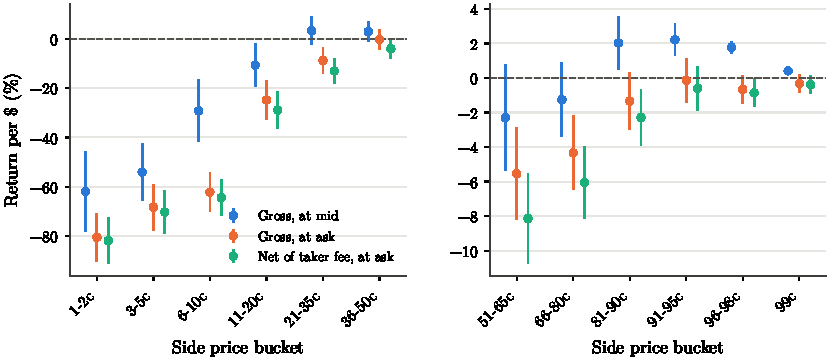
\includegraphics[width=\textwidth]{figures/fig_xs_returns.pdf}
\caption{Return per dollar by side-price bucket, all groups, market-weighted, pre-event leads
pooled: gross at the mid, gross at the ask, and net of the exact taker fee at the ask. Bars are
95\% confidence intervals clustered by event. The two panels share buckets but not the vertical
scale.}\label{fig:xs-returns}
\end{figure}

\begin{table}[!htbp]
\centering
\begin{threeparttable}
\caption{Calibration and returns by price bucket, all groups}\label{tab:xs-bucket}
\scriptsize
\begin{tabular}{@{}lrrrrrrr@{}}
\toprule
Bucket & Sides & Events & $\bar\q$ (\cents) & Win (\%) & Gross, mid (\%) & Gross, ask (\%) & Net, ask (\%) \\
\midrule
% source: data/research/flb_xs/tables/calibration.json:All.mkt
1-2c & 26{,}184 & 2{,}118 & 0.87 & 0.38 & $-62.0$ ($-7.5$) & $-80.6$ & $-81.8$ ($-17.3$) \\
3-5c & 9{,}521 & 2{,}007 & 3.53 & 1.67 & $-54.1$ ($-9.1$) & $-68.3$ & $-70.3$ ($-15.7$) \\
6-10c & 4{,}847 & 1{,}707 & 7.53 & 5.52 & $-29.2$ ($-4.5$) & $-62.2$ & $-64.4$ ($-17.1$) \\
11-20c & 6{,}366 & 1{,}919 & 15.18 & 13.73 & $-10.6$ ($-2.4$) & $-24.8$ & $-28.9$ ($-7.6$) \\
21-35c & 8{,}230 & 2{,}146 & 27.63 & 28.52 & $+3.4$ ($1.2$) & $-8.7$ & $-13.0$ ($-5.0$) \\
36-50c & 6{,}978 & 2{,}018 & 42.68 & 43.92 & $+3.0$ ($1.4$) & $-0.2$ & $-3.9$ ($-1.9$) \\
51-65c & 6{,}996 & 2{,}058 & 57.93 & 56.59 & $-2.3$ ($-1.5$) & $-5.5$ & $-8.1$ ($-6.2$) \\
66-80c & 8{,}254 & 2{,}150 & 72.95 & 72.02 & $-1.3$ ($-1.2$) & $-4.3$ & $-6.1$ ($-5.6$) \\
81-90c & 6{,}485 & 1{,}939 & 85.42 & 87.15 & $+2.0$ ($2.6$) & $-1.3$ & $-2.3$ ($-2.8$) \\
91-95c & 5{,}548 & 1{,}826 & 93.20 & 95.26 & $+2.2$ ($4.7$) & $-0.1$ & $-0.6$ ($-0.9$) \\
96-98c & 10{,}721 & 2{,}041 & 96.96 & 98.68 & $+1.8$ ($9.7$) & $-0.7$ & $-0.9$ ($-2.1$) \\
99c & 23{,}854 & 1{,}983 & 99.24 & 99.65 & $+0.4$ ($5.6$) & $-0.3$ & $-0.4$ ($-1.4$) \\
\bottomrule
\end{tabular}
\begin{tablenotes}\footnotesize
\item YES and NO sides of every usable pre-event quote, market-weighted. $\bar\q$: mean mid price of
the side; Win: weighted share that paid out. Returns per dollar; the ask columns bucket sides by
the ask. $t$-statistics clustered by event in parentheses.
\end{tablenotes}
\end{threeparttable}
\end{table}

\subsubsection{Horizon}\label{sec:res-xs-horizon}

Pooled across groups, the slope is $\xsTermAllThirtyDBeta$ at 30 days ($t=\xsTermAllThirtyDBetaT$),
$\xsTermAllSevenDBeta$ at 7 days, $\xsTermAllOneDBeta$ at 24 hours ($t=\xsTermAllOneDBetaT$) and
$\xsTermAllOneHBeta$ at one hour ($t=\xsTermAllOneHBetaT$) (\cref{tab:xs-term,fig:xs-term}). Prices
do not become calibrated as resolution approaches; if anything, the bias steepens in the last day.
The pattern is clearest in Entertainment, where the slope is $\xsTermEntThirtyDBeta$ at 30 days,
$\xsTermEntSevenDBeta$ at 7 days and $\xsTermEntOneDBeta$--$\xsTermEntSixHBeta$ within the last
day ($t=\xsTermEntOneDBetaT$ at 24 hours). Within other groups the cells are noisier and the
confidence intervals overlap across leads.

\citet{pageclemen2013} find calibration good at short horizons and a bias in long-dated contracts,
which they attribute to the cost of tying up capital. Kalshi's short horizons do not remove the bias.
This finding does not support a purely capital-cost explanation. The capital term of the no-arbitrage band
in \cref{sec:framework} scales with the horizon, so it predicts a bias that shrinks towards zero at short
leads. At one hour the opportunity cost of capital is negligible, yet the slope is at least as steep
as at 30 days.

\paragraph{Sports pre-game and in-play.}
For sports events with a scheduled start time in the ticker, the horizon is exact. Their pre-game
prices are close to calibrated: $\hat\beta=\xsTermSportsStartOneDBeta$ at 24 hours,
$\xsTermSportsStartSixHBeta$ at 6 hours and $\xsTermSportsStartOneHBeta$ one hour before the start
($t=\xsTermSportsStartOneHBetaT$). Half an hour into the game the slope is
$\xsTermSportsStartInHalfBeta$ ($t=\xsTermSportsStartInHalfBetaT$), and it is
$\xsTermSportsStartInOneBeta$ and $\xsTermSportsStartInTwoBeta$ one and two hours in. None of these
differs significantly from one. Longshots still lose in play: sides priced at most 10\cents{},
such as a team trailing late, return \xsInplayLsMid\% per dollar at the mid ($t=\xsInplayLsMidT$).
Most in-play longshot quotes sit in the 1--2\cents{} bucket, where the tick floor binds
(\cref{sec:res-xs-limits}).

\begin{figure}[!htbp]
\centering
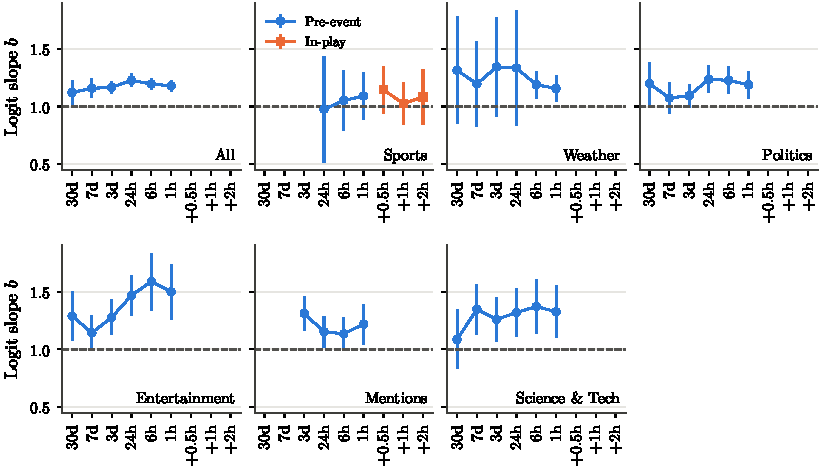
\includegraphics[width=\textwidth]{figures/fig_xs_term.pdf}
\caption{Term structure of the calibration slope $\hat\beta$ by group, from 30 days to 1 hour before
the scheduled time. The sports panel uses events with a start time in the ticker, before and 0.5, 1
and 2 hours after the start (in-play). One quote per market and lead; 95\% confidence intervals
clustered by event. The dashed line ($\beta=1$) is calibration.}\label{fig:xs-term}
\end{figure}

\begin{table}[!htbp]
\centering
\begin{threeparttable}
\caption{Calibration slope by lead and group}\label{tab:xs-term}
\scriptsize
\setlength{\tabcolsep}{3.5pt}
\begin{tabular}{@{}lrrrrrrr@{}}
\toprule
Lead & All & Sports & Weather & Politics & Entert. & Mentions & Sci.\,\&\,Tech \\
\midrule
% source: data/research/flb_xs/tables/term.json
1h & 1.180 & 1.092 & 1.158 & 1.190 & 1.501 & 1.218 & 1.326 \\
 & ($7.1$) & ($0.9$) & ($2.7$) & ($3.2$) & ($4.1$) & ($2.5$) & ($2.8$) \\[1pt]
6h & 1.196 & 1.053 & 1.190 & 1.228 & 1.590 & 1.135 & 1.372 \\
 & ($7.7$) & ($0.4$) & ($3.1$) & ($3.8$) & ($4.7$) & ($1.8$) & ($3.1$) \\[1pt]
24h & 1.229 & 0.976 & 1.335 & 1.238 & 1.469 & 1.151 & 1.320 \\
 & ($7.8$) & ($-0.1$) & ($1.3$) & ($3.9$) & ($5.3$) & ($2.2$) & ($2.9$) \\[1pt]
3d & 1.166 &  & 1.345 & 1.096 & 1.278 & 1.311 & 1.259 \\
 & ($5.9$) &  & ($1.6$) & ($1.9$) & ($3.6$) & ($4.1$) & ($2.7$) \\[1pt]
7d & 1.159 &  & 1.197 & 1.074 & 1.143 &  & 1.348 \\
 & ($3.8$) &  & ($1.0$) & ($1.1$) & ($1.8$) &  & ($3.1$) \\[1pt]
30d & 1.123 &  & 1.316 & 1.200 & 1.288 &  & 1.085 \\
 & ($2.3$) &  & ($1.3$) & ($2.1$) & ($2.6$) &  & ($0.6$) \\[1pt]
in-play 0.5h &  & 1.146 &  &  &  &  &  \\
 &  & ($1.4$) &  &  &  &  &  \\[1pt]
in-play 1h &  & 1.026 &  &  &  &  &  \\
 &  & ($0.3$) &  &  &  &  &  \\[1pt]
in-play 2h &  & 1.083 &  &  &  &  &  \\
 &  & ($0.7$) &  &  &  &  &  \\[1pt]
\bottomrule
\end{tabular}
\begin{tablenotes}\footnotesize
\item $\hat\beta$ of~\eqref{eq:xs-logit}, one quote per market and lead, market-weighted;
$t_{\beta=1}$ clustered by event in parentheses. The Sports column uses only events with a start
time in the ticker, so that the horizon is exact; in-play rows are 0.5, 1 and 2 hours after that
start. Cells with fewer than 100 quotes or 30 events are blank.
\end{tablenotes}
\end{threeparttable}
\end{table}

\subsubsection{Contract structure}\label{sec:res-xs-structure}

\Cref{tab:xs-structure,fig:xs-structure} compare the four contract structures. Multi-outcome
events and deadline contracts are the most biased; ladder legs and stand-alone binaries the least.

\paragraph{Deadline contracts.}
``By date'' contracts have $\hat\beta=\xsStDeadlineBeta$ ($t=\xsStDeadlineBetaT$), and their
longshots return \xsStDeadlineRegLsMid\% per dollar ($t=\xsStDeadlineRegLsMidT$). Only multi-outcome longshots lose more per dollar.

\paragraph{Ladder legs.}
Strike-ladder legs have $\hat\beta=\xsStLadderBeta$ ($t=\xsStLadderBetaT$). Their tails return
\xsStLadderRegLsMid\% per dollar at the mid ($t=\xsStLadderRegLsMidT$), and the body (35--65\cents)
\xsStLadderRegBodyMid\%. The implied distribution has tails that are too fat relative to outcomes,
the cross-strike form of the bias, but the tail loss is smaller than in the other structures.

\paragraph{Binaries.}
Stand-alone binaries have $\hat\beta=\xsStBinaryBeta$ ($t=\xsStBinaryBetaT$).

\paragraph{Multi-outcome events.}
Mutually exclusive events with at least three outcomes have $\hat\beta=\xsStMultiBeta$
($t=\xsStMultiBetaT$). \Cref{tab:xs-multi} shows where their mispricing sits.
\begin{itemize}
\item \emph{Overround.} Summed asks exceed one by \xsMeMultiOverAsk\% ($t=\xsMeMultiOverAskT$) in
      multi-outcome events and by \xsMeTwoOverAsk\% in two-leg events. That is the cost of buying the
      whole book, and it is mostly spread. In two-leg events the mids sum to one (\xsMeTwoOverMid\%).
      In multi-outcome events the mids themselves exceed one by \xsMeMultiOverMid\%
      ($t=\xsMeMultiOverMidT$): even at the mid, the book is overpriced.
\item \emph{Shin's insider share.} The median $\shinz$ is \xsMeMultiZMedian{} in multi-outcome and
      \xsMeTwoZMedian{} in two-leg events. These are of the same order as estimates for bookmaker
      markets \citep{shin1993}, but on an exchange $\shinz$ mostly restates the bid--ask spread.
      Median $\shinz$ is similar across groups (\cref{tab:xs-shin-group}).
\item \emph{The field.} Per event and lead, the legs priced at or below 10\cents{} cost
      \xsMeMultiFieldPrice\cents{} together and pay out \xsMeMultiFieldWin\cents{} on average: an
      overpricing of \xsMeMultiFieldGap\cents{} ($t=\xsMeMultiFieldGapT$). Realised minus price is
      \xsMeMultiRankOneEmid\cents{} for the favourite leg ($t=\xsMeMultiRankOneEmidT$) and
      \xsMeMultiRankSixEmid\cents{} for legs ranked sixth or lower ($t=\xsMeMultiRankSixEmidT$).
\end{itemize}
\Cref{fig:xs-multi} in the appendix plots these errors by rank.
Shin's adjustment moves probability from longshots to favourites, but with $\shinz$ near
\xsMeMultiZMedian{} the move is small. The field remains overpriced by \xsMeMultiFieldShinGap\cents{}
after the adjustment ($t=\xsMeMultiFieldShinGapT$), and the Brier score barely changes
(\xsMeMultiBrierMid{} raw, \xsMeMultiBrierShin{} Shin). The longshot overpricing in these events is
therefore not the price protection against insiders that Shin's model implies. It is closer to many
small bets spread over the field. Within multi-outcome events the slope does not rise with the number
of outcomes: it is $\xsMultiLegsThreeBeta$ for 3--5 legs, $\xsMultiLegsSixBeta$ for 6--10,
$\xsMultiLegsElevenBeta$ for 11--20 and $\xsMultiLegsTwentyOneBeta$ for more.

\begin{table}[!htbp]
\centering
\begin{threeparttable}
\caption{The bias by contract structure}\label{tab:xs-structure}
\scriptsize
\setlength{\tabcolsep}{3.5pt}
\begin{tabular}{@{}lrrrrrrrr@{}}
\toprule
 & & & & \multicolumn{3}{c}{Gross, at mid} & \multicolumn{2}{c}{Net, at ask} \\
\cmidrule(lr){5-7}\cmidrule(l){8-9}
Structure & Markets & Events & $\hat\beta$ & \LS & 35--65\cents & \FAV & \LS & \FAV \\
\midrule
% source: data/research/flb_xs/tables/structure.json
Binary & 6{,}028 & 2{,}644 & 1.120 & $-64.1$ & $+0.2$ & $+1.7$ & $-79.0$ & $-0.0$ \\
 &  &  & ($3.7$) & ($-9.0$) & ($0.4$) & ($6.4$) & ($-17.8$) & ($-0.0$) \\[2pt]
Multi-outcome & 3{,}441 & 474 & 1.283 & $-71.8$ & $+0.6$ & $+1.1$ & $-84.4$ & $+0.4$ \\
 &  &  & ($4.4$) & ($-8.3$) & ($0.6$) & ($7.2$) & ($-18.1$) & ($0.6$) \\[2pt]
Ladder leg & 7{,}029 & 1{,}030 & 1.118 & $-30.9$ & $+0.4$ & $+0.9$ & $-61.6$ & $-1.4$ \\
 &  &  & ($2.9$) & ($-2.3$) & ($0.9$) & ($3.9$) & ($-8.8$) & ($-2.9$) \\[2pt]
Deadline & 2{,}509 & 644 & 1.224 & $-68.3$ & $+3.3$ & $+0.9$ & $-81.1$ & $-1.1$ \\
 &  &  & ($3.9$) & ($-10.7$) & ($2.4$) & ($4.0$) & ($-20.0$) & ($-1.4$) \\[2pt]
\bottomrule
\end{tabular}
\begin{tablenotes}\footnotesize
\item Structures as defined in \cref{sec:method-xs}. Returns per dollar (\%) of sides in three price
regions; market-weighted; pre-event leads pooled; $t$-statistics clustered by event in parentheses
($t_{\beta=1}$ under $\hat\beta$).
\end{tablenotes}
\end{threeparttable}
\end{table}

\begin{figure}[!htbp]
\centering
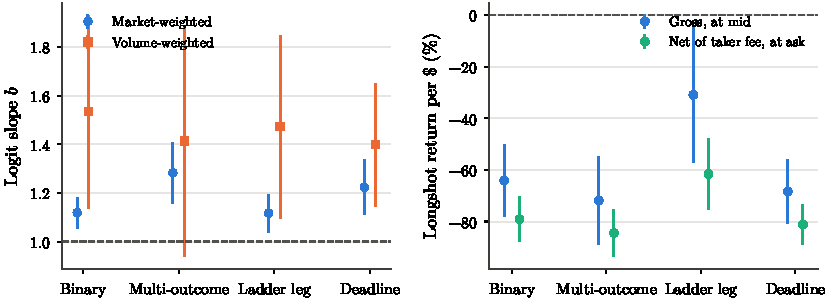
\includegraphics[width=\textwidth]{figures/fig_xs_structure.pdf}
\caption{Contract structure. Left: calibration slope, market- and volume-weighted. Right: return per
dollar on longshot sides ($\q\le10\cents$), gross at the mid and net of the taker fee at the ask.
95\% confidence intervals clustered by event.}\label{fig:xs-structure}
\end{figure}

\begin{table}[!htbp]
\centering
\begin{threeparttable}
\caption{Mutually exclusive events: overround, Shin $\shinz$ and where the mispricing sits}\label{tab:xs-multi}
\scriptsize
\setlength{\tabcolsep}{3.5pt}
\begin{tabular}{@{}lrrrrrrrr@{}}
\toprule
 & Events & Event-leads & Legs & $\sum a-1$ (\%) & $\sum p-1$ (\%) & $\sum b-1$ (\%) & Mean $\shinz$ & Median $\shinz$ \\
\midrule
% source: data/research/flb_xs/tables/structure.json:multi_outcome
Two-leg events & 740 & 2{,}009 & 2 & $+2.8$ ($41.3$) & $-0.1$ ($-3.2$) & $-3.0$ & 0.030 & 0.020 \\
Multi-outcome events ($\geq 3$ legs) & 381 & 1{,}289 & 4 & $+9.7$ ($16.6$) & $+2.3$ ($7.8$) & $-5.2$ & 0.025 & 0.017 \\
\bottomrule
\end{tabular}

\vspace{6pt}
\begin{tabular}{@{}lrrrrrr@{}}
\toprule
Leg rank & Legs & Mid (\cents) & Win (\%) & Win $-$ mid (\cents) & Win $-$ normalised (\cents) & Win $-$ Shin (\cents) \\
\midrule
% source: data/research/flb_xs/tables/structure.json:multi_outcome.multi (by_rank, field)
1 (favourite) & 1{,}289 & 68.4 & 69.8 & $+1.46$ ($0.8$) & $+3.08$ ($1.6$) & $+3.33$ ($1.7$) \\
2 & 1{,}289 & 18.2 & 16.4 & $-1.80$ ($-1.1$) & $-1.55$ ($-0.9$) & $-1.65$ ($-1.0$) \\
3-5 & 2{,}565 & 6.8 & 6.5 & $-0.33$ ($-0.4$) & $-0.24$ ($-0.3$) & $-0.34$ ($-0.4$) \\
6+ & 2{,}933 & 0.9 & 0.4 & $-0.55$ ($-3.8$) & $-0.47$ ($-3.3$) & $-0.44$ ($-3.1$) \\
\midrule
Field ($\leq 10\cents$ legs) & 762 & 9.7 & 5.4 & $-4.34$ ($-3.4$) & $-3.77$ ($-3.0$) & $-3.97$ ($-3.2$) \\
\bottomrule
\end{tabular}
\begin{tablenotes}\footnotesize
\item Top: events flagged mutually exclusive by Kalshi with every leg quoted at the lead and
exactly one leg settling YES; one observation per event and lead. $a$, $p$, $b$: YES ask, mid and
bid; $\shinz$ from the asks via~\eqref{eq:xs-shin}. Bottom: legs of events with at least three
legs, ranked by mid within the event and lead. Normalised: mid divided by the event's sum of mids.
Shin: $\hat p_k(\shinz)$. Field: per event and lead, all legs priced at or below 10\cents{} together
(their summed price against the number that win). $t$-statistics clustered by event in parentheses.
\end{tablenotes}
\end{threeparttable}
\end{table}

\subsubsection{Liquidity and calendar time}\label{sec:res-xs-liquidity}

\paragraph{Liquidity.}
The bias is not confined to thin markets (\cref{fig:xs-liq}, \cref{tab:xs-liq}). Across
within-group terciles of trailing 7-day volume, the slope is $\xsLiqVolLowBeta$, $\xsLiqVolMidBeta$
and $\xsLiqVolHighBeta$ ($t=\xsLiqVolHighBetaT$ in the top tercile). Across open-interest terciles it
is $\xsLiqOiLowBeta$, $\xsLiqOiMidBeta$ and $\xsLiqOiHighBeta$, and across spread terciles
$\xsLiqSpreadLowBeta$ (tightest), $\xsLiqSpreadMidBeta$ and $\xsLiqSpreadHighBeta$ (widest). Longshot
returns at the mid are, if anything, more negative in the most active tercile: \xsLiqVolHighLsMid\%,
against \xsLiqVolLowLsMid\% in the least active. Volume-weighted estimates are steeper than all
terciles (\cref{sec:res-xs-size}). The very largest markets, which dominate volume-weighted averages
but are a small part of the top tercile, are the most biased.

\paragraph{Calendar time.}
The slope is above one in \xsCalBetaAboveOne{} of the \xsCalNQtr{} quarters from \xsCalFirstQtr{} to
\xsCalLastQtr{} (\cref{fig:xs-liq,tab:xs-cal}).
\begin{itemize}
\item Before 2025 the venue was small (about \xsVenueEarlyMkts{} in-scope markets a quarter in 2022),
      and the quarterly slopes are noisy, ranging from $\xsCalEarlyMin$ to $\xsCalEarlyMax$.
\item From 2025, as sports listings took the venue to \xsVenuePeakMkts{} settled markets in
      \xsVenuePeakQtr, the slope settles between $\xsCalRecentMin$ and $\xsCalRecentMax$ in all
      \xsCalRecentN{} quarters.
\end{itemize}
Growth by three orders of magnitude neither removed the bias nor visibly reduced it. Whatever capital entered on the other side was not enough to remove it.

\begin{figure}[!htbp]
\centering
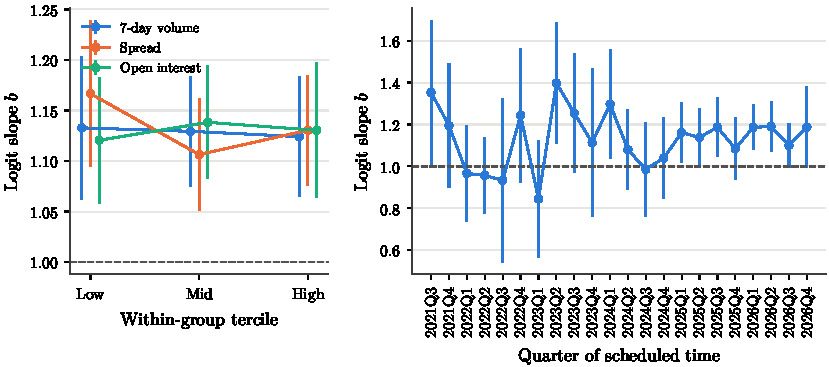
\includegraphics[width=\textwidth]{figures/fig_xs_liq_calendar.pdf}
\caption{Left: calibration slope by within-group tercile of 7-day volume, quoted spread and open
interest at the quote. Right: calibration slope by quarter of the scheduled time, all groups. Both
market-weighted, pre-event leads pooled; 95\% confidence intervals clustered by event.}\label{fig:xs-liq}
\end{figure}

\subsubsection{Fees, the tick and the limits to arbitrage}\label{sec:res-xs-limits}

\paragraph{Fees.}
Kalshi's taker fee is $0.07\,\q(1-\q)$ per contract, or $7(1-\q)$\% per dollar staked, so it is
almost flat per dollar for longshots (\cref{fig:xs-limits}, left). Kalshi computes the fee per fill to
\$0.000001 and rebates rounding over-payment \citep{kalshirounding}, so the exact fee is the fee
paid. Under a rule that rounded each order up to the cent, a single 1\cents{} contract would pay a
1\cents{} fee, 100\% of the stake; the figure shows this case for comparison. Net of fees and the half-spread, longshot
returns fall from \xsAllLsMid\% to \xsAllLsNet\% (\cref{tab:xs-group}). Fees and spread thus deepen the
longshot buyer's loss without changing its sign.

\paragraph{Taking the other side.}
The arbitrageur's question is whether buying the favourite side of every longshot pays
(\cref{tab:xs-limits}, bottom). At the mid it returns \xsOtherAllMid\% per dollar ($t=\xsOtherAllMidT$).
As a taker at the ask, net of fees, it returns \xsOtherAllTakerNet\% ($t=\xsOtherAllTakerNetT$): the
spread and fee absorb the whole premium. Resting at the bid as a maker would return \xsOtherAllMakerNet\%
($t=\xsOtherAllMakerNetT$) if every order filled at the quote. That is an upper bound: fills on resting
orders are adversely selected (\cref{sec:res-flow}).

\paragraph{The no-arbitrage band.}
\Cref{fig:xs-limits} (right) sets the mispricing per contract against the cost of trading against it.
\begin{itemize}
\item In the longshot buckets, price minus realised frequency is \xsBandBOneMis, \xsBandBThreeMis{}
      and \xsBandBSixMis{} cents per contract for 1--2, 3--5 and 6--10\cents.
\item The taker's cost (half-spread plus fee on the opposite side) is \xsBandBOneCost,
      \xsBandBThreeCost{} and \xsBandBSixCost{} cents.
\item The mispricing lies inside the taker band in \xsBandInside{} of \xsBandN{} buckets; in the three
      longshot buckets it takes up \xsBandShareMin--\xsBandShareMax\% of the band.
\end{itemize}
The longshot overpricing thus sits close to the edge of the band: most of the cost of removing it,
and no more. This is the classic limit to arbitrage \citep{shleifervishny1997}, here
created by the spread and the fee schedule rather than by capital constraints. The capital term of
the band in \cref{sec:framework} adds little at these horizons: at a 5\%
annual cost of capital, holding a 95\cents{} favourite for 30 days costs about 0.4\cents{} per
contract, and for one day about 0.01\cents.

\paragraph{The tick floor.}
The floor binds often.
\begin{itemize}
\item \xsFloorShareEither\% of quotes have a side priced at or below 2\cents, and \xsFloorSharePinned\%
      sit at the floor with no bid and a 1\cents{} ask.
\item Sides pinned there win \xsFloorPinnedWin\% of the time against a 0.5\cents{} mid. A contract worth
      about a tenth of a cent cannot be quoted lower.
\item Splitting the 1--2\cents{} bucket's loss of \xsFloorAllLoss{} cents per contract,
      \xsFloorAllMechShare\% is mechanical, the loss of quotes at the floor.
\item For a taker paying a 1--2\cents{} ask, the mechanical share is \xsFloorTakerMechShare\%: the
      1\cents{} ask alone costs nearly a cent against a win rate of \xsFloorTakerWin\%.
\end{itemize}
The rest of the 1--2\cents{} loss comes from prices above the floor. Only \xsSubcentShare\% of
markets quote on a 0.1\cents{} grid, too few for a clean comparison.

\begin{figure}[!htbp]
\centering
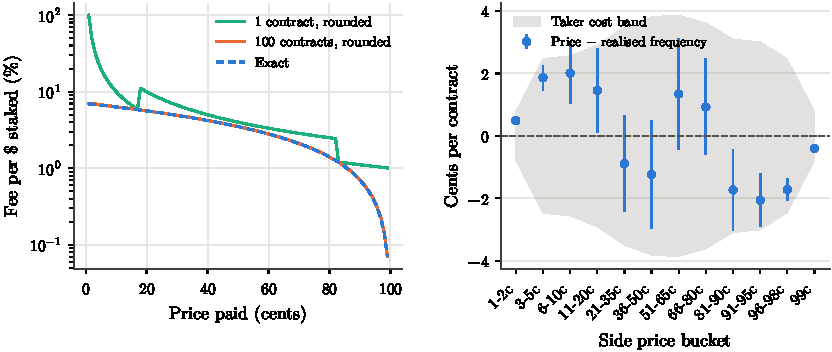
\includegraphics[width=\textwidth]{figures/fig_xs_limits.pdf}
\caption{Limits to arbitrage. Left: Kalshi taker fee per dollar staked against the price paid,
exact and rounded up to the cent for one order of 1 or 100 contracts (log scale). Right: mispricing
per contract at the mid (side price minus realised frequency, with 95\% confidence intervals
clustered by event) against the cost of trading against it as a taker (half-spread plus the taker
fee on the opposite side, shaded), by bucket of the side price.}\label{fig:xs-limits}
\end{figure}

\begin{table}[!htbp]
\centering
\begin{threeparttable}
\caption{The tick floor and the other side of longshots}\label{tab:xs-limits}
\scriptsize
\setlength{\tabcolsep}{3.5pt}
\begin{tabular}{@{}lrrrrrrr@{}}
\toprule
 & Sides & Price (\cents) & Win (\%) & Loss (\cents) & Mechanical (\cents) & Share & Return (\%) \\
\midrule
% source: data/research/flb_xs/tables/limits.json:floor
All 1--2\cents{} sides (1\cents{} grid) & 25{,}800 & 0.87 & 0.38 & 0.49 & 0.22 & 45\% & $-61.6$ ($-7.4$) \\
\quad at the floor (mid 0.5\cents) & 15{,}747 & 0.50 & 0.13 & 0.37 & 0.37 & 100\% & $-73.5$ ($-7.5$) \\
\quad above the floor & 10{,}053 & 1.44 & 0.77 & 0.67 & 0.00 & 0\% & $-43.3$ ($-3.7$) \\
0--2\cents{} sides, 0.1\cents{} grid & 384 & 0.75 & 0.00 & 0.75 & 0.01 & 1\% & $-100.0$  \\
Taker at a 1--2\cents{} ask & 20{,}948 & 1.25 & 0.29 & 0.95 & 0.65 & 68\% & $-81.6$ ($-17.1$) \\
\bottomrule
\end{tabular}

\vspace{6pt}
\begin{tabular}{@{}lrrrrr@{}}
\toprule
Buying the favourite side & Sides & Gross, mid (\%) & Gross, ask (\%) & Taker net (\%) & Maker net (\%) \\
\midrule
% source: data/research/flb_xs/tables/limits.json:other_side
All groups & 40{,}552 & $+1.11$ ($9.8$) & $-0.27$ ($-0.9$) & $-0.49$ ($-1.7$) & $+2.64$ ($21.3$) \\
Sports & 9{,}108 & $+1.11$ ($4.8$) & $+0.06$ ($0.1$) & $-0.17$ ($-0.2$) & $+2.58$ ($9.8$) \\
Weather & 3{,}905 & $+1.51$ ($4.0$) & $+0.05$ ($0.1$) & $-0.19$ ($-0.3$) & $+3.41$ ($8.6$) \\
Politics & 11{,}768 & $+0.52$ ($2.2$) & $-1.38$ ($-2.5$) & $-1.59$ ($-2.9$) & $+1.95$ ($7.8$) \\
Entertainment & 8{,}939 & $+1.36$ ($6.9$) & $+0.16$ ($0.2$) & $-0.06$ ($-0.1$) & $+2.97$ ($13.1$) \\
Mentions & 1{,}918 & $+1.63$ ($3.4$) & $+0.77$ ($0.9$) & $+0.49$ ($0.6$) & $+2.92$ ($5.5$) \\
Science \& Tech & 4{,}572 & $+1.16$ ($3.7$) & $-0.20$ ($-0.3$) & $-0.40$ ($-0.5$) & $+2.57$ ($7.3$) \\
Other & 342 & $+2.85$ ($5.7$) & $+2.66$ ($2.9$) & $+2.42$ ($2.6$) & $+4.40$ ($8.1$) \\
\bottomrule
\end{tabular}
\begin{tablenotes}\footnotesize
\item Top: sides priced at most 2\cents. Loss: price minus realised win rate, per contract.
Mechanical: the loss of sides quoted at the floor (mid 0.5\cents{} with no bid, or a 1\cents{} ask
for takers), $\max(\text{floor}-\text{win},0)$, times their weight share. Return: gross per dollar at
the mid, or net at the ask for the taker row. Bottom: buying the favourite side ($\q\ge 90\cents$ at
the mid) of every quote: at the mid; at the ask as a taker, gross and net of the taker fee; and
resting at the bid as a maker, net of the maker fee where the series charges one. The maker column
assumes a fill at the quote and ignores adverse selection, so it is an upper bound. Market-weighted;
$t$-statistics clustered by event in parentheses.
\end{tablenotes}
\end{threeparttable}
\end{table}

\subsubsection{Robustness}\label{sec:res-xs-robust}

The appendix collects the robustness checks (\cref{tab:xs-robust,tab:xs-cluster}).
\begin{itemize}
\item \emph{Sample halves.} Splitting at the median observation date (\xsRobSplit) gives
      $\hat\beta=\xsRobFirstBeta$ ($t=\xsRobFirstBetaT$) and $\xsRobSecondBeta$ ($t=\xsRobSecondBetaT$),
      and longshot returns of \xsRobFirstLsMid\% and \xsRobSecondLsMid\%. The slope exceeds one in
      \xsRobFirstGroupsAboveOne{} of \xsRobFirstGroups{} groups in the first half and
      \xsRobSecondGroupsAboveOne{} of \xsRobSecondGroups{} in the second.
\item \emph{Without the tick-floor buckets.} Dropping quotes with a mid at or below 2\cents{} or at or
      above 98\cents{} leaves $\hat\beta=\xsRobInnerBeta$ ($t=\xsRobInnerBetaT$). The slope is
      therefore not an artefact of the floor.
\item \emph{Other filters and weights.} Restricting to spreads of at most 5\cents{}
      ($\hat\beta=\xsRobSpreadBeta$) or quotes at most a day old ($\xsRobFreshBeta$), or reweighting
      by the inverse sampling probability ($\xsRobDesignBeta$, $t=\xsRobDesignBetaT$), changes little.
\item \emph{Clustering.} The test of $\beta=1$ has $t=\xsCluMarketBetaT$ when clustered by market,
      $\xsCluSeriesBetaT$ by series and $\xsCluMonthBetaT$ by calendar month.
\end{itemize}

\subsubsection{Mechanical and behavioural components}\label{sec:res-xs-summary}

The measures above separate the components that \cref{sec:framework} distinguishes.
\begin{itemize}
\item \emph{Mechanical.} The tick floor explains about half of the loss in the cheapest bucket
      (\xsFloorAllMechShare\% at the mid, \xsFloorTakerMechShare\% for a taker at the ask). Fees and
      spreads deepen buyers' losses and make the remaining mispricing uneconomic to trade against:
      the longshot overpricing lies inside the taker band, close to its edge. In this sense the bias
      survives fees for the buyer and does not survive them for the arbitrageur.
\item \emph{Not only mechanical.} The slope is $\xsRobInnerBeta$ without the floor buckets. It does
      not shrink at short horizons, where capital costs vanish. It is as strong where volume and open
      interest are high as where they are low, and it is present in every group and in both halves of
      the sample. Mechanics set the band; something else keeps prices near its edge.
\item \emph{Not insiders.} In multi-outcome events, Shin's $\shinz$ is about \xsMeMultiZMedian{} and
      largely a restatement of the spread, and the Shin adjustment leaves the field overpriced. This
      is contrary to the information hypothesis of \cref{sec:framework}.
\item \emph{Consistent with demand for lottery-like payoffs.} The bias is steepest in multi-outcome
      fields, in deadline contracts and in entertainment, where outcomes have no external anchor. It
      is weakest in politics and in pre-game sports with a known start, where polls and bookmaker
      lines provide one. This pattern is consistent with the preference and belief-dispersion
      explanations of \cref{sec:framework}, although the cross-group differences are modest. \Cref{sec:res-flow,sec:res-wallets} ask who is on each side of
      these trades.
\end{itemize}
